% CS631 Advanced Programming in the UNIX Environment
% Author: Jan Schaumann <jschauma@netmeister.org>
% $Id: slides.tex,v 1.2 2004/07/28 23:12:36 jschauma Exp $
\special{! TeXDict begin /landplus90{true}store end }

\documentclass[xga]{xdvislides}
\usepackage[landscape]{geometry}
\usepackage{graphics}
\usepackage{graphicx}
\usepackage{colordvi}
\usepackage{tabularx}
\usepackage{listings}

\newcommand{\smallish}{\fontsize{18}{18}\selectfont}

\begin{document}
\setfontphv

%%% Headers and footers
\lhead{\slidetitle}
\chead{CS631 - Advanced Programming in the UNIX Environment}
\rhead{Slide \thepage}
\lfoot{\Gray{Lecture 06: Process Groups, Sessions, Signals}}
\cfoot{\relax}
\rfoot{\Gray{\today}}

\vspace*{\fill}
\begin{center}
	\Hugesize
		CS631 - Advanced Programming in the UNIX Environment\\
		-- \\
		Process Groups, Sessions, Signals
	\hspace*{5mm}\blueline\\ [1em]
	\Normalsize
		Department of Computer Science\\
		Stevens Institute of Technology\\
		Jan Schaumann\\
		\verb+jschauma@stevens.edu+\\
		\verb+https://stevens.netmeister.org/631/+
\end{center}
\vspace*{\fill}

\subsection{Code reading}
\vspace{1in}
\\

\Huge
A volunteer, please...
\Normalsize

\subsection{Login Process}
\small
\begin{verbatim}
[...]
total memory = 768 MB
avail memory = 732 MB
timecounter: Timecounters tick every 10.000 msec
mainbus0 (root)
[...]
boot device: xbd3
root on xbd3a dumps on xbd3b
mountroot: trying lfs...
mountroot: trying ffs...
root file system type: ffs
init: copying out path `/sbin/init' 11
[...]
Starting local daemons:.
Starting sendmail.
Starting sshd.
Starting snmpd.
Starting cron.

NetBSD/amd64 (panix.netmeister.org) (console)

login: jschauma
Password:
Last login: Sat Sep 10 14:27:56 2011 on console
Copyright (c) 1982, 1986, 1989, 1991, 1993
    The Regents of the University of California.  All rights reserved.

NetBSD 5.0.2 (PANIX-VC) #2: Tue Oct 19 16:30:57 EDT 2010

Welcome to NetBSD!

$
\end{verbatim}
\Normalsize



\subsection{Login Process}
\begin{center}
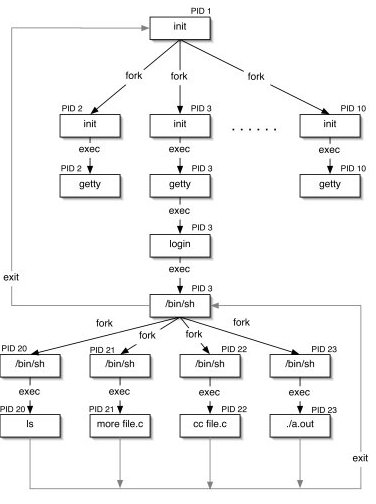
\includegraphics[scale=0.7]{pics/process-tree.eps} \\
\end{center}



\subsection{Login Process}
\begin{itemize}
	\item init(8)
		\begin{itemize}
			\item reads {\tt /etc/ttys}
		\end{itemize}
\end{itemize}

\subsection{Login Process}
\begin{itemize}
	\item init(8)
		\begin{itemize}
			\item reads {\tt /etc/ttys}
		\end{itemize}
	\item getty(8)
		\begin{itemize}
			\item opens terminal
			\item prints ``login: ''
			\item reads username
		\end{itemize}
\end{itemize}

\subsection{Login Process}
\begin{itemize}
	\item init(8)
		\begin{itemize}
			\item reads {\tt /etc/ttys}
		\end{itemize}
	\item getty(8)
		\begin{itemize}
			\item opens terminal
			\item prints ``login: ''
			\item reads username
		\end{itemize}
	\item login(1)
		\begin{itemize}
			\item getpass(3), encrypt, compare to getpwnam(3)
		\end{itemize}
\end{itemize}

\subsection{Login Process}
\begin{itemize}
	\item init(8)
		\begin{itemize}
			\item reads {\tt /etc/ttys}
		\end{itemize}
	\item getty(8)
		\begin{itemize}
			\item opens terminal
			\item prints ``login: ''
			\item reads username
		\end{itemize}
	\item login(1)
		\begin{itemize}
			\item getpass(3), encrypt, compare to getpwnam(3)
			\item register login in system databases
		\end{itemize}
\end{itemize}

\subsection{Login Process}
\begin{itemize}
	\item init(8)
		\begin{itemize}
			\item reads {\tt /etc/ttys}
		\end{itemize}
	\item getty(8)
		\begin{itemize}
			\item opens terminal
			\item prints ``login: ''
			\item reads username
		\end{itemize}
	\item login(1)
		\begin{itemize}
			\item getpass(3), encrypt, compare to getpwnam(3)
			\item register login in system databases
			\item read/display various files
		\end{itemize}
\end{itemize}

\subsection{Login Process}
\begin{itemize}
	\item init(8)
		\begin{itemize}
			\item reads {\tt /etc/ttys}
		\end{itemize}
	\item getty(8)
		\begin{itemize}
			\item opens terminal
			\item prints ``login: ''
			\item reads username
		\end{itemize}
	\item login(1)
		\begin{itemize}
			\item getpass(3), encrypt, compare to getpwnam(3)
			\item register login in system databases
			\item read/display various files
			\item initgroups(3)/setgid(2), initialize environment
		\end{itemize}
\end{itemize}

\subsection{Login Process}
\begin{itemize}
	\item init(8)
		\begin{itemize}
			\item reads {\tt /etc/ttys}
		\end{itemize}
	\item getty(8)
		\begin{itemize}
			\item opens terminal
			\item prints ``login: ''
			\item reads username
		\end{itemize}
	\item login(1)
		\begin{itemize}
			\item getpass(3), encrypt, compare to getpwnam(3)
			\item register login in system databases
			\item read/display various files
			\item initgroups(3)/setgid(2), initialize environment
			\item chown(2) terminal device
		\end{itemize}
\end{itemize}

\subsection{Login Process}
\begin{itemize}
	\item init(8)
		\begin{itemize}
			\item reads {\tt /etc/ttys}
		\end{itemize}
	\item getty(8)
		\begin{itemize}
			\item opens terminal
			\item prints ``login: ''
			\item reads username
		\end{itemize}
	\item login(1)
		\begin{itemize}
			\item getpass(3), encrypt, compare to getpwnam(3)
			\item register login in system databases
			\item read/display various files
			\item initgroups(3)/setgid(2), initialize environment
			\item chown(2) terminal device
			\item chdir(2) to new home directory
		\end{itemize}
\end{itemize}

\subsection{Login Process}
\begin{itemize}
	\item init(8)
		\begin{itemize}
			\item reads {\tt /etc/ttys}
		\end{itemize}
	\item getty(8)
		\begin{itemize}
			\item opens terminal
			\item prints ``login: ''
			\item reads username
		\end{itemize}
	\item login(1)
		\begin{itemize}
			\item getpass(3), encrypt, compare to getpwnam(3)
			\item register login in system databases
			\item read/display various files
			\item initgroups(3)/setgid(2), initialize environment
			\item chdir(2) to new home directory
			\item chown(2) terminal device
			\item setuid(2) to user's uid, exec(3) shell
		\end{itemize}
\end{itemize}



\subsection{Login Process}
Let's revisit the process relationships for a login:
\vspace*{\fill}
\begin{center}
\begin{tabular}[width=.75\texwidth]{l c l l}
kernel & $\Rightarrow$ & init(8) & \# explicit creation\\
\end{tabular}
\end{center}
\vspace*{\fill}

\subsection{Login Process}
Let's revisit the process relationships for a login:
\vspace*{\fill}
\begin{center}
\begin{tabular}[width=.75\texwidth]{l c l l}
kernel & $\Rightarrow$ & init(8) & \# explicit creation\\
\\
init(8) & $\Rightarrow$ & getty(8) & \# fork(2) \\
\end{tabular}
\end{center}
\vspace*{\fill}

\subsection{Login Process}
Let's revisit the process relationships for a login:
\vspace*{\fill}
\begin{center}
\begin{tabular}[width=.75\texwidth]{l c l l}
kernel & $\Rightarrow$ & init(8) & \# explicit creation\\
\\
init(8) & $\Rightarrow$ & getty(8) & \# fork(2) \\
\\
getty(8) & $\Rightarrow$ & login(1) & \# exec(3) \\
\end{tabular}
\end{center}
\vspace*{\fill}

\subsection{Login Process}
Let's revisit the process relationships for a login:
\vspace*{\fill}
\begin{center}
\begin{tabular}[width=.75\texwidth]{l c l l}
kernel & $\Rightarrow$ & init(8) & \# explicit creation\\
\\
init(8) & $\Rightarrow$ & getty(8) & \# fork(2) \\
\\
getty(8) & $\Rightarrow$ & login(1) & \# exec(3) \\
\\
login(1) & $\Rightarrow$ & \verb+$SHELL+ & \# exec(3) \\
\end{tabular}
\end{center}
\vspace*{\fill}

\subsection{Login Process}
Let's revisit the process relationships for a login:
\vspace*{\fill}
\begin{center}
\begin{tabular}[width=.75\texwidth]{l c l l }
kernel & $\Rightarrow$ & init(8) & \# explicit creation \\
\\
init(8) & $\Rightarrow$ & getty(8) & \# fork(2) \\
\\
getty(8) & $\Rightarrow$ & login(1) & \# exec(3) \\
\\
login(1) & $\Rightarrow$ & \verb+$SHELL+ & \# exec(3) \\
\\
\verb+$SHELL+ & $\Rightarrow$ & ls(1) & \# fork(2) + exec(3) \\
\end{tabular}
\end{center}
\vspace*{\fill}

\subsection{Login Process}
\vspace*{\fill}
\begin{center}
\begin{tabular}[width=.75\texwidth]{l c l}
init(8) & \# PID 1, PPID 0, EUID 0\\
\end{tabular}
\vspace*{\fill}
\end{center}

\subsection{Login Process}
\vspace*{\fill}
\begin{center}
\begin{tabular}[width=.75\texwidth]{l c l}
init(8) & \# PID 1, PPID 0, EUID 0\\
\\
getty(8) & \# PID {\em N}, PPID 1, EUID 0\\
\end{tabular}
\vspace*{\fill}
\end{center}

\subsection{Login Process}
\vspace*{\fill}
\begin{center}
\begin{tabular}[width=.75\texwidth]{l c l}
init(8) & \# PID 1, PPID 0, EUID 0\\
\\
getty(8) & \# PID {\em N}, PPID 1, EUID 0\\
\\
login(1) & \# PID {\em N}, PPID 1, EUID 0\\
\end{tabular}
\vspace*{\fill}
\end{center}

\subsection{Login Process}
\vspace*{\fill}
\begin{center}
\begin{tabular}[width=.75\texwidth]{l c l}
init(8) & \# PID 1, PPID 0, EUID 0\\
\\
getty(8) & \# PID {\em N}, PPID 1, EUID 0\\
\\
login(1) & \# PID {\em N}, PPID 1, EUID 0\\
\\
\verb+$SHELL+ & \# PID {\em N}, PPID 1, EUID {\em U}\\
\end{tabular}
\vspace*{\fill}
\end{center}

\subsection{Login Process}
\vspace*{\fill}
\begin{center}
\begin{tabular}[width=.75\texwidth]{l c l}
init(8) & \# PID 1, PPID 0, EUID 0\\
\\
getty(8) & \# PID {\em N}, PPID 1, EUID 0\\
\\
login(1) & \# PID {\em N}, PPID 1, EUID 0\\
\\
\verb+$SHELL+ & \# PID {\em N}, PPID 1, EUID {\em U}\\
\\
ls(1) & \# PID {\em M}, PPID {\em N}, EUID {\em U}\\
\\
\end{tabular}
\vspace*{\fill}
\end{center}
\begin{center}
\verb+pstree -hapun | more+
\end{center}

\subsection{Process Groups}
\small
\setlength{\unitlength}{1mm}
\begin{center}
	\begin{picture}(150,30)
		\thinlines
		\put(0,0){\framebox(130,25){}}
		\put(10,20){{\tt \#include <unistd.h>}}
		\put(10,13){{\tt pid\_t getpgrp(void);}}
		\put(10,8){{\tt pid\_t getpgid(pid\_t {\em pid});}}
		\put(55,3){Returns: process group ID if OK, -1 otherwise}
	\end{picture}
\end{center}
\Normalsize
\begin{itemize}
	\item in addition to having a PID, each process also
		belongs to a process group (collection of processes
		assocaited with the same job / terminal)
	\item each process group has a unique process group ID
	\item process group IDs (like PIDs) are positive integers and can
		be stored in a {\tt pid\_t} data type
	\item each process group can have a process group leader
		\begin{itemize}
			\item leader identified by its process group ID == PID
			\item leader can create a new process group, create processes in the group
		\end{itemize}
	\item a process can set its (or its children's) process group using {\tt setpgid(2)}
\end{itemize}



\subsection{Process Groups}
\begin{center}
	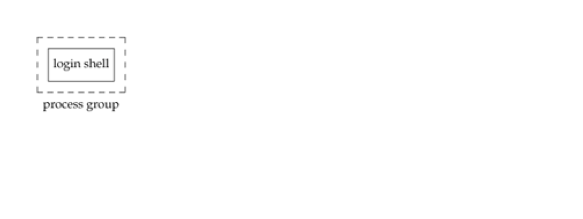
\includegraphics[angle=-90,scale=0.8]{pics/session1.eps}
\end{center}

{\em init} $\Rightarrow$ {\em login shell}
\begin{verbatim}
$
\end{verbatim}

\subsection{Process Groups}
\begin{center}
	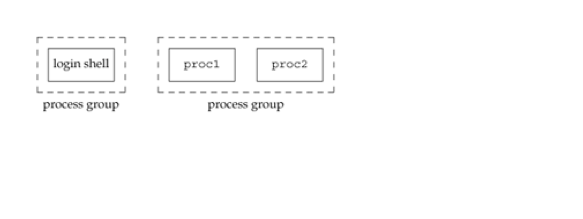
\includegraphics[angle=-90,scale=0.8]{pics/session2.eps}
\end{center}

{\em init} $\Rightarrow$ {\em login shell}
\begin{verbatim}
$ proc1 | proc2 &
[1] 10306
$
\end{verbatim}

\subsection{Process Groups}
\begin{center}
	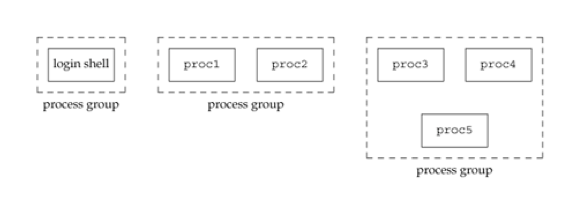
\includegraphics[angle=-90,scale=0.8]{pics/session3.eps}
\end{center}

{\em init} $\Rightarrow$ {\em login shell}
\begin{verbatim}
$ proc1 | proc2 &
[1] 10306
$ proc3 | proc4 | proc5

\end{verbatim}


\subsection{Process Groups and Sessions}
\small
\setlength{\unitlength}{1mm}
\begin{center}
	\begin{picture}(150,30)
		\thinlines
		\put(0,0){\framebox(130,22){}}
		\put(10,18){{\tt \#include <unistd.h>}}
		\put(10,10){{\tt pid\_t setsid(void);}}
		\put(30,5){Returns: process group ID if OK, -1 otherwise}
	\end{picture}
\end{center}
\Normalsize
A session is a collection of one or more process groups. \\

If the calling process is not a process group leader, this
function creates a new session.  Three things happen:
\begin{itemize}
	\item the process becomes the session leader of this new session
	\item the process becomes the process group leader of a new process group
	\item the process has no controlling terminal
\end{itemize}

\subsection{Process Groups}
\begin{center}
	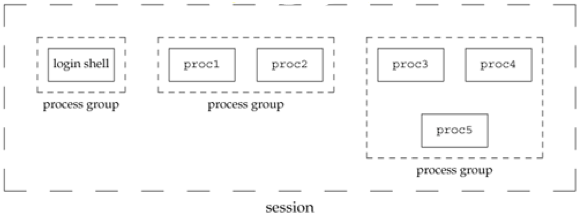
\includegraphics[angle=-90,scale=0.8]{pics/session4.eps}
\end{center}

{\em init} $\Rightarrow$ {\em login shell}
\begin{verbatim}
$ proc1 | proc2 &
[1] 10306
$ proc3 | proc4 | proc5

\end{verbatim}

\subsection{Process Groups and Sessions}
\begin{center}
	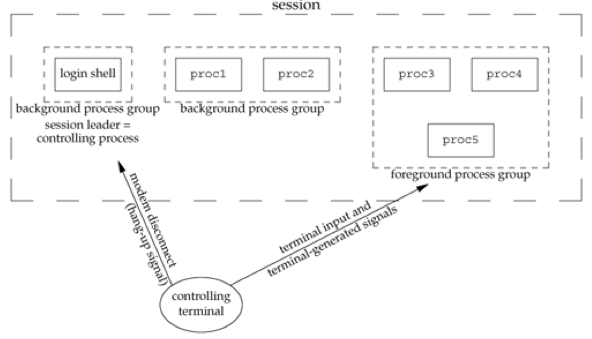
\includegraphics[angle=-90,scale=0.75]{pics/session5.eps}
\end{center}

{\em init} $\Rightarrow$ {\em login shell}
\begin{verbatim}
$ proc1 | proc2 &
[1] 10306
$ proc3 | proc4 | proc5
\end{verbatim}


\subsection{Process Groups and Sessions}
\begin{center}
	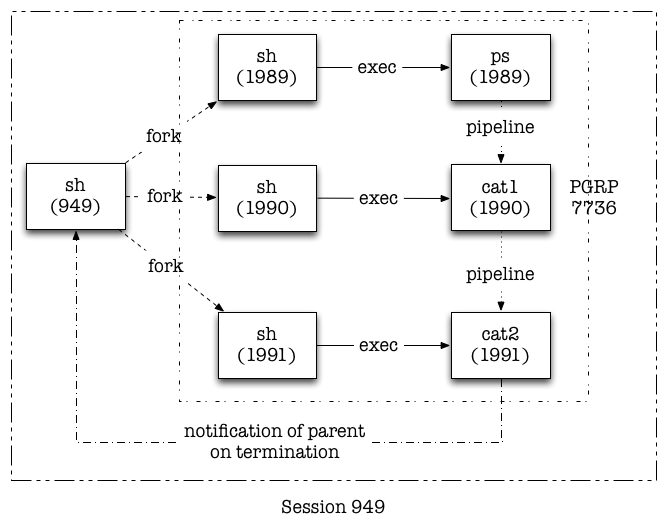
\includegraphics[angle=-90,scale=0.6]{pics/pscat.eps}
\end{center}
\begin{verbatim}
$ ( ps -o pid,ppid,pgid,sid,comm; sleep 1; ) | ./cat1 | ./cat2
  PID  PPID  PGRP  SESS COMMAND
 1989   949  7736   949 ps
 1990   949  7736   949 cat1
 1988   949  7736   949 cat2
  949 21401   949   949 ksh
\end{verbatim}


\subsection{Job Control}
\begin{center}
	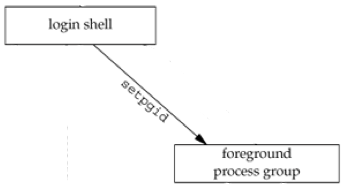
\includegraphics[angle=-90,scale=0.75]{pics/jc3.eps}
\end{center}
\addvspace{.5in}
\begin{verbatim}
$ ps -o pid,ppid,pgid,sid,comm
  PID  PPID  PGRP  SESS COMMAND
24251 24250 24251 24251 ksh
24620 24251 24620 24251 ps
$
\end{verbatim}

\subsection{Job Control}
\begin{center}
	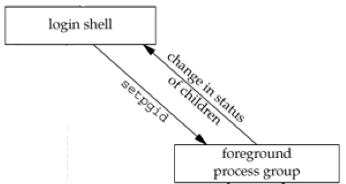
\includegraphics[angle=-90,scale=0.75]{pics/jc4.eps}
\end{center}
\addvspace{.5in}
\begin{verbatim}
$ ps -o pid,ppid,pgid,sid,comm
  PID  PPID  PGRP  SESS COMMAND
24251 24250 24251 24251 ksh
24620 24251 24620 24251 ps
$ echo $?
0
$
\end{verbatim}

\subsection{Job Control}
\begin{center}
	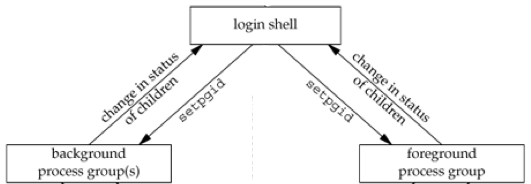
\includegraphics[angle=-90,scale=0.75]{pics/jc2.eps}
\end{center}
\begin{verbatim}
$ /bin/sleep 30 &
[1]	24748
$ ps -o pid,ppid,pgid,sid,comm
  PID  PPID  PGRP  SESS COMMAND
24251 24250 24251 24251 ksh
24748 24251 24748 24251 sleep
24750 24251 24750 24251 ps
$
[1] +  Done     /bin/sleep 30 &
$
\end{verbatim}

\subsection{Job Control}
\begin{center}
	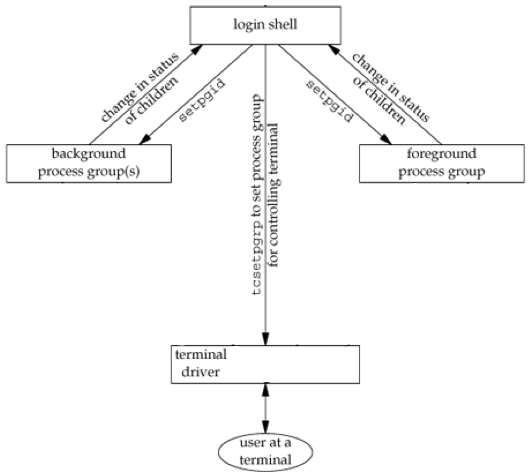
\includegraphics[angle=-90,scale=0.75]{pics/jc6.eps}
\end{center}

\subsection{Job Control}
\begin{center}

\newsavebox\fgio
\begin{lrbox}{\fgio}
	\begin{minipage}[t]{\textwidth}
		\begin{verbatim}
$ cat >file
Input from terminal,
Output to terminal.
^D
$ cat file
Input from terminal,
Output to terminal.
$ cat >/dev/null
Input from terminal,
Output to /dev/null.
Waiting forever...
Or until we send an interrupt signal.
^C
$
\end{verbatim}
	\end{minipage}
\end{lrbox}

\renewcommand{\tabularxcolumn}[1]{>{\arraybackslash}m{#1}}
\begin{tabularx}{\textwidth}{l r }
\begin{minipage}[b]{0.5\textwidth}
\usebox\fgio
\end{minipage} &
		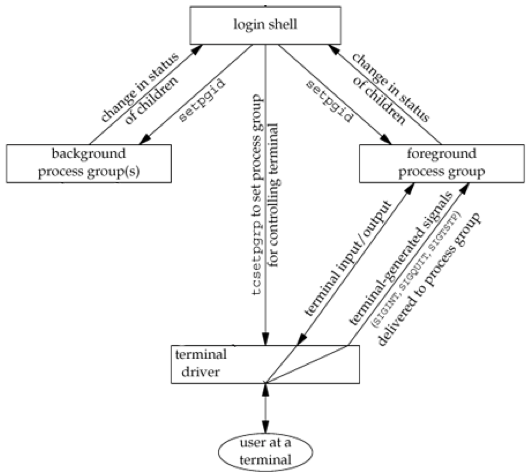
\includegraphics[angle=-90,scale=0.6]{pics/jc5.eps}
	\end{tabularx}
\end{center}

\subsection{Job Control}
\begin{center}

\newsavebox\bgio
\begin{lrbox}{\bgio}
	\begin{minipage}[t]{\textwidth}
		\begin{verbatim}
$ cat file &
[1]	2056
$ Input from terminal,
Output to terminal.

[1] +  Done             cat file &
$ stty tostop
$ cat file &
[1]	4655
$
[1] + Stopped(SIGTTOU)  cat file &
$ fg
cat file
Input from terminal,
Output to terminal.
$
\end{verbatim}
	\end{minipage}
\end{lrbox}

\renewcommand{\tabularxcolumn}[1]{>{\arraybackslash}m{#1}}
\begin{tabularx}{\textwidth}{l r }
\begin{minipage}[b]{0.5\textwidth}
\usebox\bgio
\end{minipage} &
		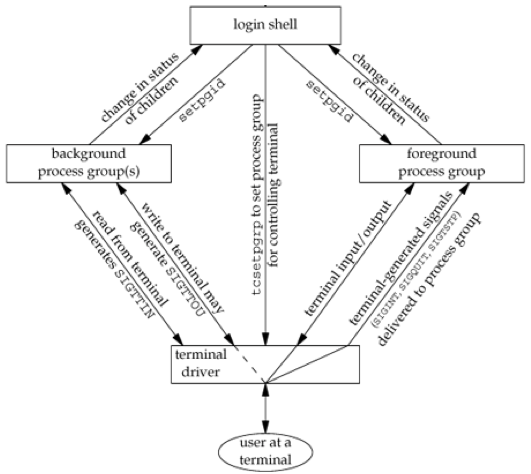
\includegraphics[angle=-90,scale=0.6]{pics/jc1.eps}
	\end{tabularx}
\end{center}

\subsection{Signals}
\begin{center}
	
\includegraphics[angle=-90,scale=0.6]{pics/shithappens.eps}
\end{center}

\subsection{Signal Concepts}

Signals are a way for a process to be notified of asynchronous events. Some
examples:

\begin{itemize}
	\item a timer you set has gone off ({\tt SIGALRM})
	\item some I/O you requested has occurred ({\tt SIGIO})
	\item a user resized the terminal "window" ({\tt SIGWINCH})
	\item a user disconnected from the system ({\tt SIGHUP})
	\item ...
\end{itemize}

See also: {\tt signal(2)/signal(3)/signal(7)} (note: these man pages vary
significantly across platforms!)
\subsection{Signal Concepts}
Besides the asynchronous events listed previously, there are many ways to
generate a signal:

\begin{itemize}
	\item terminal generated signals (user presses a key combination which causes
		the terminal driver to generate a signal)
\end{itemize}

\subsection{Signal Concepts}
Besides the asynchronous events listed previously, there are many ways to
generate a signal:

\begin{itemize}
	\item terminal generated signals (user presses a key combination which causes
		the terminal driver to generate a signal)
	\item hardware exceptions (divide by 0, invalid memory references, etc)
\end{itemize}

\subsection{Signal Concepts}
Besides the asynchronous events listed previously, there are many ways to
generate a signal:

\begin{itemize}
	\item terminal generated signals (user presses a key combination which causes
		the terminal driver to generate a signal)
	\item hardware exceptions (divide by 0, invalid memory references, etc)
	\item {\tt kill(1)} allows a user to send any signal to any process (if the
		user is the owner or superuser)
\end{itemize}

\subsection{Signal Concepts}
Besides the asynchronous events listed previously, there are many ways to
generate a signal:

\begin{itemize}
	\item terminal generated signals (user presses a key combination which causes
		the terminal driver to generate a signal)
	\item hardware exceptions (divide by 0, invalid memory references, etc)
	\item {\tt kill(1)} allows a user to send any signal to any process (if the
		user is the owner or superuser)
	\item {\tt kill(2)} (a system call, not the unix command) performs the
		same task
\end{itemize}


\subsection{Signal Concepts}
Besides the asynchronous events listed previously, there are many ways to
generate a signal:

\begin{itemize}
	\item terminal generated signals (user presses a key combination which causes
		the terminal driver to generate a signal)
	\item hardware exceptions (divide by 0, invalid memory references, etc)
	\item {\tt kill(1)} allows a user to send any signal to any process (if the
		user is the owner or superuser)
	\item {\tt kill(2)} (a system call, not the unix command) performs the
		same task
	\item software conditions (other side of a pipe no longer exists, urgent data
		has arrived on a network file descriptor, etc.)
\end{itemize}

\subsection{{\tt kill(2)} and {\tt raise(3)}}
\small
\setlength{\unitlength}{1mm}
\begin{center}
	\begin{picture}(150,27)
		\thinlines
		\put(0,0){\framebox(130,27){}}
		\put(10,22){{\tt \#include <sys/types.h>}}
		\put(10,17){{\tt \#include <signal.h>}}
		\put(10,10){{\tt int kill(pid\_t {\em pid}, int {\em signo});}}
		\put(10,5){{\tt int raise(int {\em signo});}}
	\end{picture}
\end{center}
\Normalsize

\begin{itemize}
	\item {\em pid $>$ 0} -- signal is sent to the process whose PID is {\tt pid}
	\item {\em pid == 0} -- signal is sent to all processes whose process
		group ID equals the process group ID of the sender
	\item {\em pid == -1} -- POSIX.1 leaves this undefined, BSD defines it
		(see {\tt kill(2)})
\end{itemize}

\subsection{Signal Concepts}
Once we get a signal, we can do one of several things:

\begin{itemize}
	\item Ignore it. (note: there are some signals which we CANNOT or SHOULD NOT
		ignore)
\end{itemize}

\subsection{Signal Concepts}
Once we get a signal, we can do one of several things:

\begin{itemize}
	\item Ignore it. (note: there are some signals which we CANNOT or SHOULD NOT
		ignore)
	\item Catch it. That is, have the kernel call a function which we define
		whenever the signal occurs.
\end{itemize}


\subsection{Signal Concepts}
Once we get a signal, we can do one of several things:

\begin{itemize}
	\item Ignore it. (note: there are some signals which we CANNOT or SHOULD NOT
		ignore)
	\item Catch it. That is, have the kernel call a function which we define
		whenever the signal occurs.
	\item Accept the default. Have the kernel do whatever is defined as the
		default action for this signal
\end{itemize}


\subsection{Signal Concepts}
\begin{verbatim}
$ cc -Wall ../01-intro/simple-shell.c
$ ./a.out
$$ ^C
$ echo $?
130
$ cc -Wall ../01-intro/simple-shell2.c
$ ./a.out
$$ ^C
Caught SIGINT!

$$
\end{verbatim}

\subsection{{\tt signal(3)}}
\small
\setlength{\unitlength}{1mm}
\begin{center}
	\begin{picture}(150,22)
		\thinlines
		\put(0,0){\framebox(130,22){}}
		\put(10,17){{\tt \#include <signal.h>}}
		\put(10,10){{\tt void (*signal(int {\em signo}, void (*func)(int)))(int);}}
		\put(30,3){Returns: previous disposition of signal if OK, {\tt SIG\_ERR} otherwise}
	\end{picture}
\end{center}
\Normalsize

\subsection{{\tt signal(3)}}
\small
\setlength{\unitlength}{1mm}
\begin{center}
	\begin{picture}(150,22)
		\thinlines
		\put(0,0){\framebox(130,22){}}
		\put(10,17){{\tt \#include <signal.h>}}
		\put(10,10){{\tt void (*signal(int {\em signo}, void (*func)(int)))(int);}}
		\put(30,3){Returns: previous disposition of signal if OK, {\tt SIG\_ERR} otherwise}
	\end{picture}
\end{center}
\Normalsize
{\em func} can be:
\begin{itemize}
	\item {\tt SIG\_IGN} which requests that we ignore the signal {\tt signo}
	\item {\tt SIG\_DFL} which requests that we accept the default action for signal {\tt signo}
	\item or the address of a function which should catch or handle a signal
\end{itemize}

\subsection{Signal Examples}
\begin{verbatim}
$ cc -Wall siguser.c
$ ./a.out
^Z
$ bg
$ ps | grep a.ou[t]
11106 ttys002    0:00.00 ./a.out
$ kill -USR1 11106
received SIGUSR1
$ kill -USR2 11106
received SIGUSR2
$ kill -INT 11106
$
[2]-  Interrupt               ./a.out
$
\end{verbatim}

\subsection{Program Startup}

When a program is {\tt exec}ed, the status of all signals is either {\em
default} or {\em ignore}.

\subsection{Program Startup}

When a program is {\tt exec}ed, the status of all signals is either {\em
default} or {\em ignore}.
\\

When a process {\tt fork(2)}s, the child inherits the parent's signal
dispositions.

\subsection{Program Startup}

When a program is {\tt exec}ed, the status of all signals is either {\em
default} or {\em ignore}.
\\

When a process {\tt fork(2)}s, the child inherits the parent's signal
dispositions.
\\

A limitation of the {\tt signal(3)} function is that we can only determine the
current disposition of a signal by {\em changing} the disposition.

\subsection{{\tt sigaction(2)}}
\small
\setlength{\unitlength}{1mm}
\begin{center}
	\begin{picture}(200,20)
		\thinlines
		\put(0,0){\framebox(180,20){}}
		\put(10,15){{\tt \#include <signal.h>}}
		\put(10,8){{\tt int sigaction(int {\em signo}, const struct sigaction *{\em act}, struct sigaction *{\em oact});}}
	\end{picture}
\end{center}
\Normalsize

This function allows us to examine or modify the action associated with a
particular signal.
\\

\begin{verbatim}
  struct sigaction {
        void (*sa_handler)();   /* addr of signal handler, or
                                   SIG_IGN or SIG_DFL */
        sigset_t sa_mask;       /* additional signals to block */
        int sa_flags;           /* signal options */
  };
\end{verbatim}

{\tt signal(3)} is (nowadays) commonly implemented via {\tt sigaction(2)}.

\subsection{More advanced signal handling via signal sets}
\begin{itemize}
	\item {\tt int sigemptyset(sigset\_t *set)} -- intialize a signal set to be empty
	\item {\tt int sigfillset(sigset\_t *set)} -- initialize a signal set to contain all signals
	\item {\tt int sigaddset(sigset\_t *set, int signo)}
	\item {\tt int sigdelset(sigset\_t *set, int signo)}
	\item {\tt int sigismember(sigset\_t *set, int signo)}
\end{itemize}

\subsection{Resetting Signal Handlers}
{\em Note}: on some systems, invocation of the handler {\em resets} the
disposition to {\tt SIG\_DFL}!

\begin{verbatim}
$ cc -DSLEEP=3 -Wall pending.c
$ ./a.out
=> Establishing initial signal hander via signal(3).
^\sig_quit: caught SIGQUIT (1), now sleeping
sig_quit: exiting (1)
=> Time for a second interruption.
^\sig_quit: caught SIGQUIT (2), now sleeping
sig_quit: exiting (2)
=> Establishing a resetting signal hander via signal(3).
^\sig_quit_reset: caught SIGQUIT (3), sleeping and resetting.
sig_quit_reset: restored SIGQUIT handler to default.
=> Time for a second interruption.
^\Quit: 3
$
\end{verbatim}

\subsection{Signal Queuing}
Signals arriving while a handler runs are queued.
\begin{verbatim}
$ ./a.out >/dev/null
^\sig_quit: caught SIGQUIT (1), now sleeping
^\^\^\^\^\^\sig_quit: exiting (1)
sig_quit: caught SIGQUIT (2), now sleeping
^\^\^\^\sig_quit: exiting (2)
sig_quit: caught SIGQUIT (3), now sleeping
^\sig_quit: exiting (3)
sig_quit: caught SIGQUIT (4), now sleeping
sig_quit: exiting (4)
[...]
\end{verbatim}

(Note that "simultaneously" delivered signals may be "merged" into one.)

\subsection{Signal Queuing}
Signals arriving while a handler runs are queued. \\
Unless they are blocked.

\begin{verbatim}
$ ./a.out
[...]
=> Establishing a resetting signal hander via signal(3).
^\sig_quit_reset: caught SIGQUIT (1), sleeping and resetting.
sig_quit_reset: restored SIGQUIT handler to default.
=> Time for a second interruption.
=> Blocking delivery of SIGQUIT...
=> Now going to sleep for 3 seconds...
^\
=> Checking if any signals are pending...
=> Checking if pending signals might be SIGQUIT...
Pending SIGQUIT found.
=> Unblocking SIGQUIT...
Quit: 3
\end{verbatim}


\subsection{Signal Queuing}
Multiple identical signals are queued, but you can receive a different
signal {\em while in a signal handler}.
\begin{verbatim}
$ ./a.out >/dev/null
^\sig_quit: caught SIGQUIT (1), now sleeping
^\^\^\^\^Csig_int: caught SIGINT (2), returning immediately
sig_quit: exiting (2)
sig_quit: caught SIGQUIT (3), now sleeping
^\^\sig_quit: exiting (3)
sig_quit: caught SIGQUIT (4), now sleeping
sig_quit: exiting (4)
[...]
\end{verbatim}

\subsection{Interrupted System Calls}

Some system calls can block for long periods of time (or forever). These
include things like:

\begin{itemize}
	\item {\tt read(2)}s from files that can block (pipes, networks, terminals)
\end{itemize}

\subsection{Interrupted System Calls}

Some system calls can block for long periods of time (or forever). These
include things like:

\begin{itemize}
	\item {\tt read(2)}s from files that can block (pipes, networks, terminals)
	\item {\tt write(2)} to the same sort of files
\end{itemize}

\subsection{Interrupted System Calls}

Some system calls can block for long periods of time (or forever). These
include things like:

\begin{itemize}
	\item {\tt read(2)}s from files that can block (pipes, networks, terminals)
	\item {\tt write(2)} to the same sort of files
	\item {\tt open(2)} of a device that waits until a condition occurs (for example, a modem)
\end{itemize}



\subsection{Interrupted System Calls}

Some system calls can block for long periods of time (or forever). These
include things like:

\begin{itemize}
	\item {\tt read(2)}s from files that can block (pipes, networks, terminals)
	\item {\tt write(2)} to the same sort of files
	\item {\tt open(2)} of a device that waits until a condition occurs (for example, a modem)
	\item {\tt pause(3)}, which purposefully puts a process to sleep until a signal occurs
\end{itemize}

\subsection{Interrupted System Calls}

Some system calls can block for long periods of time (or forever). These
include things like:

\begin{itemize}
	\item {\tt read(2)}s from files that can block (pipes, networks, terminals)
	\item {\tt write(2)} to the same sort of files
	\item {\tt open(2)} of a device that waits until a condition occurs (for example, a modem)
	\item {\tt pause(3)}, which purposefully puts a process to sleep until a signal occurs
	\item certain {\tt ioctl(3)}s
	\item certain IPC functions
\end{itemize}


\subsection{Interrupted System Calls}

Some system calls can block for long periods of time (or forever). These
include things like:

\begin{itemize}
	\item {\tt read(2)}s from files that can block (pipes, networks, terminals)
	\item {\tt write(2)} to the same sort of files
	\item {\tt open(2)} of a device that waits until a condition occurs (for example, a modem)
	\item {\tt pause(3)}, which purposefully puts a process to sleep until a signal occurs
	\item certain {\tt ioctl(3)}s
	\item certain IPC functions
\end{itemize}

Catching a signal during execution of one of these calls traditionally led
to the process being aborted with an errno return of {\tt EINTR}.


\subsection{Interrupted System Calls}
Previously necessary code to handle {\tt EINTR}:
\begin{verbatim}
again:
        if ((n = read(fd, buf, BUFFSIZE)) < 0) {
                if (errno == EINTR)
                        goto again;  /* just an interrupted system call */
                /* handle other errors */
}
\end{verbatim}

Nowadays, many Unix implementations automatically restart certain system
calls.

\subsection{Interrupted System Calls}
\begin{verbatim}
$ cc -Wall eintr.c
$ ./a.out
^C
read call was interrupted
||
$ ./a.out
^\a

read call was restarted
|a|
$
\end{verbatim}

\subsection{Reentrant functions}
An example of calling nonreentrant functions from a signal handler:
\begin{verbatim}
$ cc -Wall reentrant.c; ./a.out
in signal handler
in signal handler
in signal handler
no 'root' found!
$ ./a.out
in signal handler
return value corrupted: pw_name = root
$ ./a.out
in signal handler
in signal handler
User jschauma not found!
$ ./a.out
in signal handler
in signal handler
Memory fault (core dumped)
\end{verbatim}

\subsection{Reentrant Functions}

If your process is currently handling a signal, what functions are you allowed
to use? \\

See p. 306 in Stevens for a list.


\subsection{Homework}

Read:
\begin{itemize}
	\item Controlling Terminals: {\tt tty(4)}, {\tt termios(4)}
\end{itemize}
\vspace{.5in}
Read, try, play with and understand all examples. \\

Review the discussions around an issue we discovered
in a previous class:
\begin{itemize}
	\item {\tt https://is.gd/x95eFp}
	\item {\tt https://is.gd/Rqn03R}
	\item {\tt https://is.gd/GYYE32}
\end{itemize}

(See following slides.)

\subsection{An entertaining tangent in code exploration...}
\begin{verbatim}
$ timeout 60 /bin/sh -c "ls | more"

vs

$ /bin/sh -c "timeout 60 /bin/sh -c \"ls | more\""
\end{verbatim}

\subsection{An entertaining tangent in code exploration...}
\smallish
\begin{verbatim}
$ timeout 60 /bin/sh -c "ls | more; sleep 60"

$ pstree -hapun
[...]
  |   |       `-ksh,10981
  |   |           `-sh,12044 -c timeout 60 /bin/sh -c "ls | more; sleep 30"
  |   |               `-timeout,12045 60 /bin/sh -c ls | more; sleep 30
  |   |                   `-sh,12046 -c ls | more; sleep 30
  |   |                       `-sleep,12049 30
[...]

$ ps x -o pid,ppid,pgid,sid,tpgid,stat,comm | egrep -v "(ssh|ps|egrep)"
  PID  PPID  PGID  SESS TPGID STAT COMMAND
 7676  7675  7676  7676  7676 Ss+  ksh
10981 10980 10981 10981 12044 Ss   ksh
12044 10981 12044 10981 12044 S+   sh
12045 12044 12045 10981 12044 S    timeout
12046 12045 12045 10981 12044 S    sh
12049 12046 12045 10981 12044 S    sleep
\end{verbatim}

\subsection{An entertaining tangent in code exploration...}
\smallish
\begin{verbatim}
$ /bin/sh -c timeout 60 "/bin/sh -c \"ls | more\""

$ pstree -hapun
[...]
  |   |       `-ksh,10981
  |   |           `-sh,12434 -c timeout 60 /bin/sh -c "ls | more"
  |   |               `-timeout,12435 60 /bin/sh -c ls | more
  |   |                   `-sh,12436 -c ls | more
  |   |                       |-ls,12437
  |   |                       `-more,12438
[...]

$ ps x -o pid,ppid,pgid,sid,tpgid,stat,comm | egrep -v "(ssh|ps|egrep)"
  PID  PPID  PGID  SESS TPGID STAT COMMAND
 7676  7675  7676  7676  7676 Ss+  ksh
10981 10980 10981 10981 12434 Ss   ksh
12434 10981 12434 10981 12434 S+   sh
12435 12434 12435 10981 12434 S    timeout
12436 12435 12435 10981 12434 T    sh
12437 12436 12435 10981 12434 T    ls
12438 12436 12435 10981 12434 T    more
\end{verbatim}

\subsection{An entertaining tangent in code exploration...}
Use the source, Luke!
\\

\begin{verbatim}
coreutils/src/timeout.c

  /* Ensure we're in our own group so all subprocesses can be killed.
     Note we don't just put the child in a separate group as
     then we would need to worry about foreground and background groups
     and propagating signals between them.  */
  if (!foreground)
    setpgid (0, 0);

[...]

      signal (SIGTTIN, SIG_DFL);
      signal (SIGTTOU, SIG_DFL);

      execvp (argv[0], argv);
\end{verbatim}

\subsection{An entertaining tangent in code exploration...}
Use the source, Luke!
\\

\begin{verbatim}
util-linux/text-utils/more.c

#define stty(fd,argp)  tcsetattr(fd,TCSANOW,argp)


    if (!no_tty) {
        signal(SIGQUIT, onquit);
        signal(SIGINT, end_it);
#ifdef SIGWINCH
        signal(SIGWINCH, chgwinsz);
#endif /* SIGWINCH */
        if (signal (SIGTSTP, SIG_IGN) == SIG_DFL) {
            signal(SIGTSTP, onsusp);
            catch_susp++;
        }
        stty (fileno(stderr), &otty);

\end{verbatim}



\end{document}
